\documentclass[../main.tex]{subfiles}

\begin{document}

Trong các mô hình học máy, chúng ta thường chỉ quan tâm đến một đơn vị cụ thể và huấn luyện riêng lẻ một mô hình để thực hiện tác vụ mà ta cần giải quyết. Sau bước này sẽ là tiếp tục tối ưu mô hinh cho đến khi kết quả của mô hình không còn tăng nữa. Hướng tiếp cận này đã giúp ta đạt được kết quả một mức tương đối tốt bằng việc chỉ tập trung vào một mục tiêu duy nhất. Thế nhưng điều này làm ta vô tình quên đi có những thông tin chất lượng, hữu ích từ những bài toán tương tự hoặc liên quan có thể giúp ta tăng hiệu suất của mô hình. Bằng việc chia sẻ những biểu diễn, thông tin giữa các tác vụ hay bài toán, ta có thể giúp mô hình tổng quan hóa tốt hơn trên tác vụ gốc. Đây chính là việc học đa tác vụ. 

Việc học kết hợp như vậy đã được áp dụng thành công vào một số bài toán như xử lý ngôn ngữ tự nhiên \cite{collobert2008unified}, nhận diện giọng nói \cite{deng2013new}, thị giác máy \cite{he2015proceedings}. Mô hình học này còn gọi là học kết hợp, học với những tác vụ liên quan. Tổng quan, khi thấy rằng mô hình bài toán ta đang phải tối ưu nhiều hơn 1 hàm mất mát thì có nghĩa là ta đang áp dụng học đa tác vụ, vì mỗi tác vụ tương ứng với một hàm mất mát. Hoặc kể cả khi chỉ đang tối ưu một hàm mất mát thì vẫn có thể có một tác vụ liên quan giúp cho kết quả bài toán chính tốt hơn. 

Điều này giống như khi con người muốn giải quyết một bài toán sẽ dùng đến kiến thức của những tác vụ liên quan. Ví dụ như một vận động viên điền kinh, ngoài các bài tập chạy thì họ còn phải trải qua những bài tập như giãn cơ, khởi động, xoay các khớp để giúp cơ thể linh hoạt, từ đó giúp cho việc tránh chấn thương và đạt được thể lực tốt nhất. 

Để làm rõ tư tưởng về việc kết hợp học các bài toán, ta đi vào 2 phương pháp thường được sử dụng để học đa tác vụ trong các mạng nơ-ron. Trong ngữ cảnh học sâu, việc kết hợp này thường được thực hiện qua qua việc chia sẻ cố định hoặc tùy ý các tầng ẩn. 


\begin{itemize}

\item Chia sẻ cố định các tham số 

Phương pháp này thường được sử dụng trong các mạng nơ-ron. Một vài tầng ẩn sẽ được chia sẻ giữa các tác vụ, trong khi đó giữ lại những tầng cụ thể phục vụ cho từng tác vụ riêng. 

\begin{figure}[h]
\centering
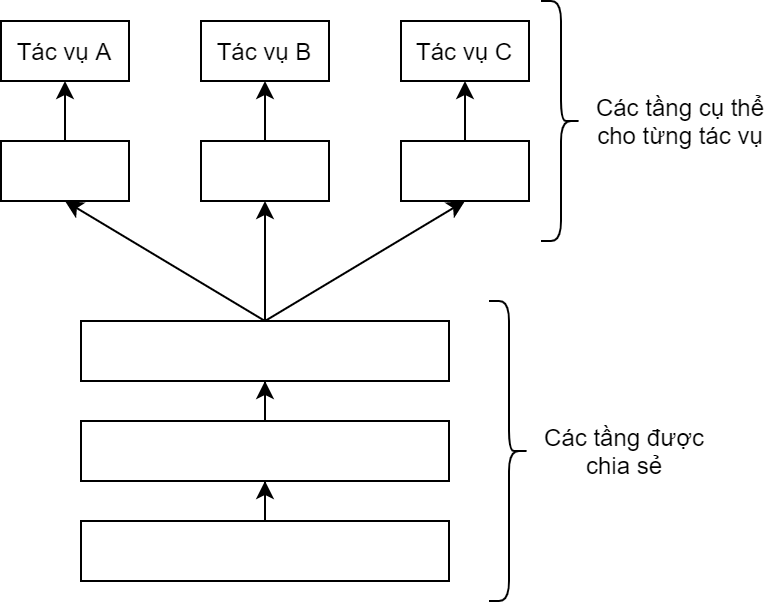
\includegraphics[scale=0.4]{02-multitask-hard}
\caption{Mô tả cấu trúc việc chia sẻ cố định các tham số}
\end{figure}

Việc chia sẻ cố định như vậy giảm đáng kể việc mô hình bị quá khớp. Điều này là rõ ràng vì càng nhiều tác vụ ta huấn luyện cùng lúc, mô hình sẽ càng phải tìm ra một biểu diễn mà tổng quát được tất cả thông tin của các tác vụ đó, vì thế nên khả năng bị quá khớp giảm đi. 

\item Chia sẻ linh hoạt giữa các tham số 

Với phương pháp này, mỗi tác vụ sẽ được giải quyết với một mô hình riêng, bộ tham số riêng. Khoảng cách giữa các tham số sau đó được chuẩn hóa để làm sao cho các tham số là gần giống nhau. 

\begin{figure}[h]
\centering
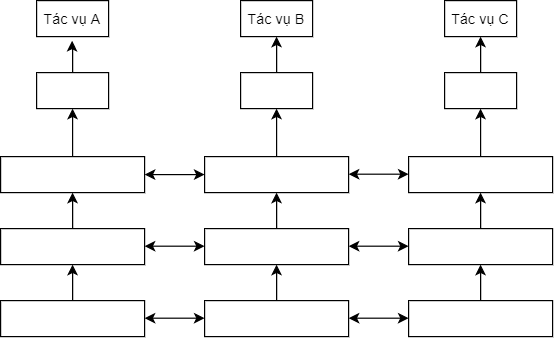
\includegraphics[scale=0.5]{02-multitask-soft}
\caption{Mô tả cấu trúc việc chia sẻ linh hoạt các tham số}
\end{figure}


\end{itemize}

Mô hình học đa tác vụ đã xuất hiện từ trước đó, tuy nhiên trong bài toán nhận diện tên thực thể Y Sinh thì chưa có nhiều thử nghiệm. \cite{crichton2017neural} đã thử nghiệm mô hình này với mạng nơ-ron sử dụng chính là CNN. Mô hình của Crichton chỉ quan tâm các đặc trưng về từ ngữ mà bỏ qua ngữ nghĩa phản ánh bởi kí tự - một điều rất cần quan tâm trong các bài toán về tên thực thể Y Sinh (ví dụ ``-ase'' thường là một từ con quan trọng cần phải cân nhắc khi nhận diện tên gene/protein). 

\end{document}